\title{VGP-2017-Poster}
%%%%%%%%%%%%%%%%%%%%%%%%%%%%%%%%%%%%%%%%%
% a0poster Portrait Poster
% LaTeX Template
% Version 1.0 (22/06/13)
%
% The a0poster class was created by:
% Gerlinde Kettl and Matthias Weiser (tex@kettl.de)
%
% This template has been downloaded from:
% http://www.LaTeXTemplates.com
%
% License:
% CC BY-NC-SA 3.0 (http://creativecommons.org/licenses/by-nc-sa/3.0/)
%
%%%%%%%%%%%%%%%%%%%%%%%%%%%%%%%%%%%%%%%%%

%-------------------------------------------------------------------------------
%	PACKAGES AND OTHER DOCUMENT CONFIGURATIONS
%-------------------------------------------------------------------------------

\documentclass[a0,portrait]{a0poster}
\usepackage{multicol} % This is so we can have multiple columns of text side-by-side
\columnsep=100pt % This is the amount of white space between the columns in the poster
\columnseprule=3pt % This is the thickness of the black line between the columns in the poster

\usepackage{xcolor}
\usepackage{tcolorbox}

\definecolor{sangertext}{RGB}{7,73,135}
\definecolor{sangersubtitletext}{RGB}{106,185,215}
\definecolor{codepurple}{rgb}{0.58,0,0.82}
\definecolor{backcolour}{rgb}{0.95,0.95,0.92}

% Sanger colour palette
\definecolor{sangerdarkblue}{RGB}{0, 72, 105}
\definecolor{sangermidblue}{RGB}{138, 187, 238}
\definecolor{sangerlightblue1}{RGB}{159, 198, 238}
\definecolor{sangerlightblue2}{RGB}{184, 210, 239}
\definecolor{sangerlightblue3}{RGB}{203, 220, 230}
\definecolor{sangerlightteal}{RGB}{176, 227, 192}
\definecolor{sangerlimegreen}{RGB}{204, 242, 132}
\definecolor{sangerlightyellow}{RGB}{255, 255, 224}
\definecolor{sangerolivegreen}{RGB}{95, 128, 17}
\definecolor{sangerdarkteal}{RGB}{5, 122, 82}
\definecolor{sangermintgreen}{RGB}{221, 246, 164}
\definecolor{sangerdarkbrown}{RGB}{132, 109, 83}
\definecolor{sangerlightbrown}{RGB}{204, 179, 118}
\definecolor{sangerdarkmustard}{RGB}{132, 93, 0}
\definecolor{sangerredbrown}{RGB}{98, 23, 0}
\definecolor{sangerorange}{RGB}{255, 114, 0}
\definecolor{sangerred}{RGB}{195, 0, 29}
\definecolor{sangerdarkred}{RGB}{141, 0, 23}
\definecolor{sangerpurple}{RGB}{124, 0, 79}

\definecolor{caecilian}{HTML}{0000ff}
\definecolor{cyprinid}{HTML}{9400d3}
\definecolor{rodent}{HTML}{17d017}
\definecolor{notothenioid}{HTML}{ff0000}
\definecolor{cichlid}{HTML}{ed22f0}
\definecolor{anabantoid}{HTML}{ff8000}

\usepackage[scaled=1.0]{helvet}

\usepackage{graphicx} % Required for including images
\graphicspath{{figures/}} % Location of the graphics files
\usepackage{booktabs} % Top and bottom rules for table
\usepackage[font=small,labelfont=bf,justification=centering]{caption} % Required for specifying captions to tables and figures
\usepackage{subcaption}
\usepackage{amsfonts, amsmath, amsthm, amssymb} % For math fonts, symbols and environments
\usepackage{wrapfig} % Allows wrapping text around tables and figures
\usepackage{enumerate}
\usepackage[hyphens]{url}
\usepackage{sidecap}
\usepackage[colorlinks,urlcolor=sangerred,linkcolor=black,citecolor=black,linktoc=all]{hyperref}
\setlength{\columnseprule}{0.01pt}
\renewcommand{\columnseprulecolor}{\color[rgb]{0.9,0.9,0.9}}

\renewcommand{\familydefault}{\sfdefault}

\setlength\heavyrulewidth{0.1pt}
\setlength\lightrulewidth{0.1pt}
\setlength{\tabcolsep}{12pt}

\setlength\labelsep   {\dimexpr\labelsep + 0.5em\relax}
\setlength\leftmargini{\dimexpr\leftmargini + 0.5em\relax}

\usepackage{sectsty}
\sectionfont{\color{sangertext}}
\subsectionfont{\color{sangersubtitletext}}

\usepackage[square,numbers]{natbib}
\usepackage[document]{ragged2e}

\begin{document}

%-------------------------------------------------------------------------------
%	POSTER HEADER
%-------------------------------------------------------------------------------

\begin{center}
\veryHuge \color{sangertext} \textbf{Scaling up reference quality assembly of vertebrate genomes} \color{sangersubtitletext}
\end{center}

\par\smallskip\noindent
\centerline{\begin{minipage}{0.975\textwidth}
\centering
\Large\color{black}
\textbf{Shane A. McCarthy}\textsuperscript{1,2},
Iliana Bista\textsuperscript{1,2},
Dirk-Dominik Dolle\textsuperscript{1},
Francesca Giordano\textsuperscript{1},
William Chow\textsuperscript{1},
Petr Danecek\textsuperscript{1},
Hannes Svardal\textsuperscript{1,2},\\
Milan Malinsky\textsuperscript{1,3},
Jingtao Lilue\textsuperscript{1},
Michelle Smith\textsuperscript{1},
Kim Judge\textsuperscript{1},
Karen Oliver\textsuperscript{1},
Mike Quail\textsuperscript{1},
Zemin Ning\textsuperscript{1},
Kerstin Howe\textsuperscript{1},
Richard Durbin\textsuperscript{1,2}\\
\vspace{0.5cm}
\normalsize
\textsuperscript{1}Wellcome Trust Sanger Institute, Hinxton, CB10 1SA, UK
\hspace{1cm}
\textsuperscript{2}Department of Genetics, University of Cambridge, Cambridge, CB2 3EH, UK\\
\textsuperscript{3}Zoological Institute, Department of Environmental Sciences, University of Basel, 4051 Basel, Switzerland
\hspace{1cm}
\end{minipage}}
\par\smallskip

\vfill

\begin{tcolorbox}[boxsep=30pt,width=0.985\textwidth,colback=sangerlightblue3,arc=20pt]
\Large\noindent\color{sangertext}
Increased read length and throughput of long read sequencing technologies such as PacBio and Oxford Nanopore are now enabling high contiguity and accuracy de novo reference assemblies for vertebrate scale genomes. During 2017 the Wellcome Trust Sanger Institute has undertaken a pilot project aiming to obtain \textbf{reference quality genome sequences} for 50-100 species and additional genome data for a similar number of related species. Our primary focus is on \textbf{fish genomes}, but we are also sequencing some \textbf{amphibian} and \textbf{mammalian} species. This initiative is part of the broader international \textbf{Vertebrate Genomes Project (VGP) }being led by the Genome 10k Consortium in collaboration with a number of other genome sequencing projects. The initial aim of the VGP is to obtain reference quality genome assemblies for \textbf{one species from every vertebrate order} over the next year or two.

\end{tcolorbox}

\vfill

\begin{center}\noindent\rule{1.0\linewidth}{0.05pt}\end{center}

%-------------------------------------------------------------------------------

\begin{multicols}{3}

%-------------------------------------------------------------------------------
%	Project overview
%-------------------------------------------------------------------------------

\vspace{0.5cm}
\begin{tcolorbox}[boxsep=20pt,width=\linewidth,colback=sangerlightyellow,arc=20pt]
\large \color{sangertext}
\begin{flushleft}
\begin{itemize}
\setlength{\itemsep}{1.5pt}
\item \textbf{$\sim$30 representatives of fish orders} for which adequate references do not currently exist.
\item multiple samples (6 references plus up to 10-20 others) within each of the following fish groups:
\begin{itemize}
	\item {\color{cyprinid}\textbf{cyprinids}} related to the zebrafish \emph{Danio rerio}.
	\item {\color{cichlid}\textbf{cichlid}} fish part of the major cichlid evolutionary radiations; recently completed sequencing of $>$1000 genomes using Illumina HiSeqX.
	\item {\color{notothenioid}\textbf{notothenioid}} fish from the Antarctic radiation.
	\item {\color{anabantoid}\textbf{anabantoid}} fish including gouramis.
\end{itemize}
\item several {\color{caecilian}\textbf{caecilian}} species representing the most basal branch of amphibians.
\item multiple {\color{rodent}\textbf{rodents}} with extreme phenotypes providing evolutionary context to mice and rats.
\end{itemize}
\end{flushleft}
\end{tcolorbox}
\vspace{0.5cm}

\vfill
\columnbreak

{\center\section*{Project overview}}

\noindent Species targetted as part of this project are summarised in the box to the left and in Figure 1. To collect these samples we are collaborating with multiple members of the Genome10k community and other evolutionary researchers.

\vspace{0.5cm}

\begin{center}
\captionsetup{type=figure}
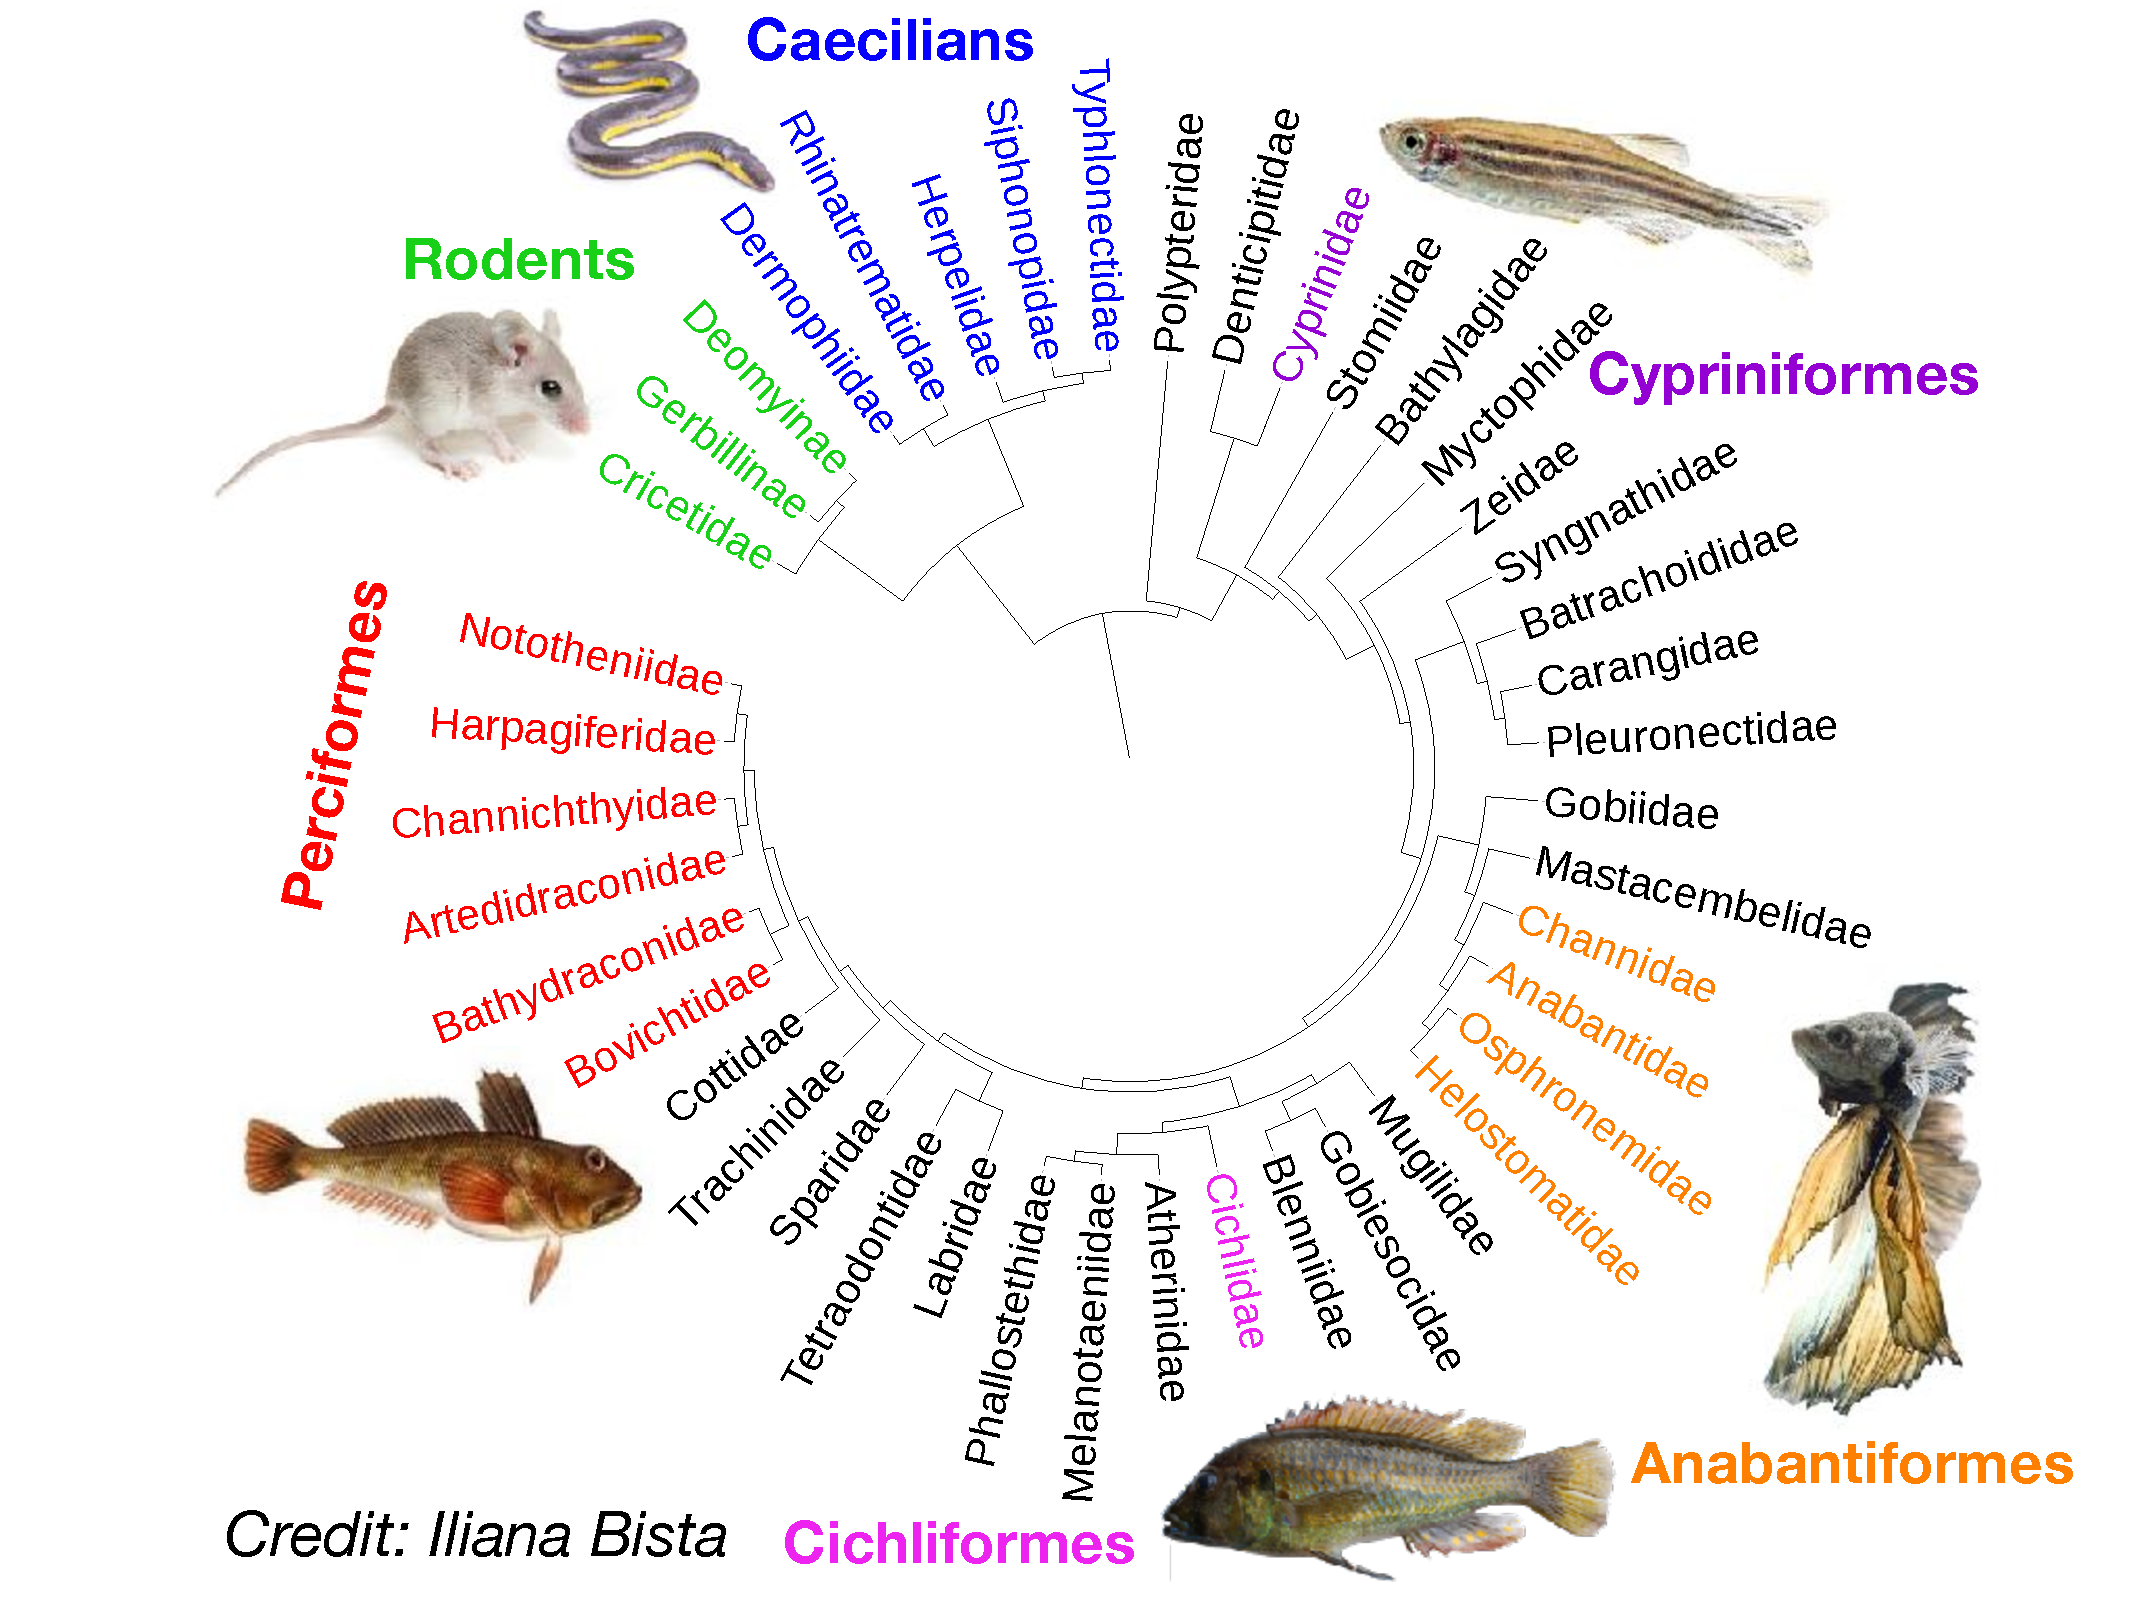
\includegraphics[width=1.0\linewidth]{images/tree-with-images.pdf}
\captionof{figure}{Highlighted are groups where we will sequence additional species for more in depth analyses.}
\end{center}

\vfill
\columnbreak

\noindent We are currently using \textbf{Pacific Biosciences Sequel}, \textbf{10X Genomics Chromium} and \textbf{BioNano Saphyr} as core technologies within existing production and R\&D pipelines at the Sanger Institute. We are evaluating others technologies including \textbf{Oxford Nanopore}. For the VGP orders, we will also generate HiC data to aid chromosome assignment and polishing.

\vspace{0.5cm}

\begin{center}
\captionsetup{type=figure}
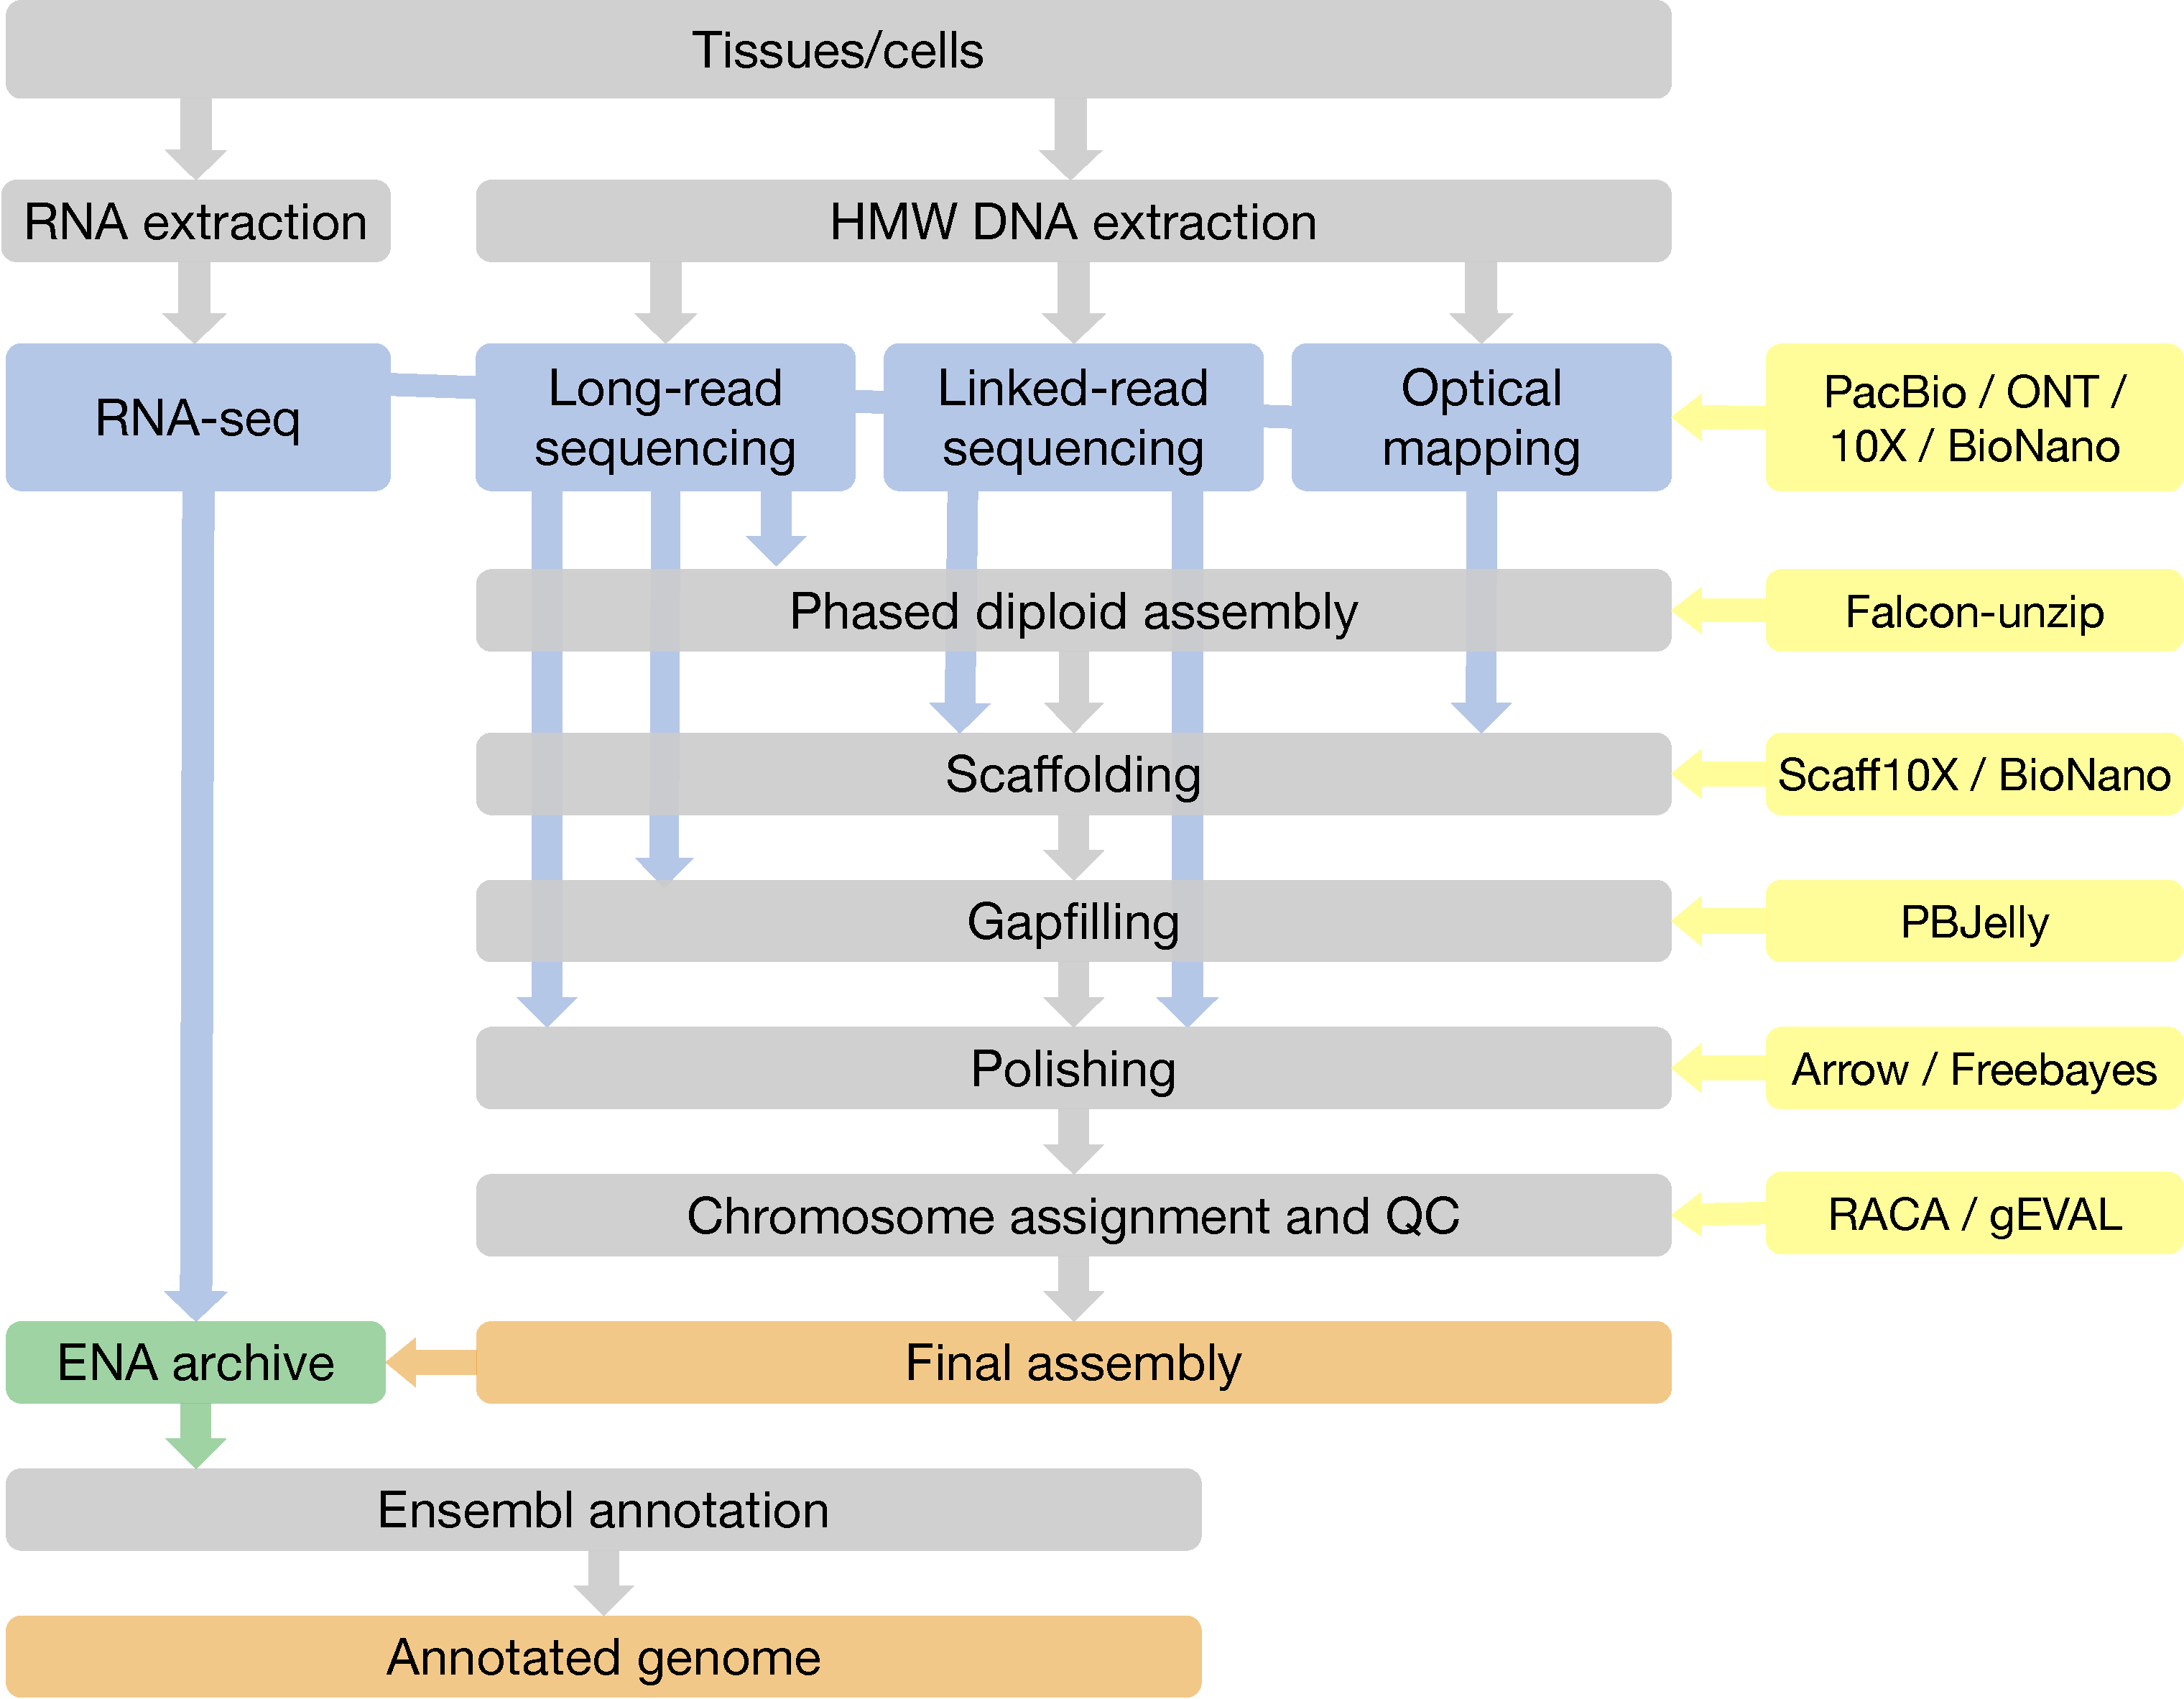
\includegraphics[width=1.0\linewidth]{images/flow.pdf}
\captionof{figure}{Data production at the Sanger for long-read reference quality de novo assemblies. We are collaborating with the European Bioinformatics Institute (EBI) to streamline data deposition into the relevant archives to enable efficient gene annotation and presentation in Ensembl.}
\end{center}

\end{multicols}

\begin{center}\noindent\rule{1.0\linewidth}{0.05pt}\end{center}

\begin{multicols}{2}

%-------------------------------------------------------------------------------
%	10X Genomics Chromium linked-read QC
%-------------------------------------------------------------------------------

\section*{10X Genomics Chromium linked-read QC}

\emph{Credit: Petr Danecek and Zemin Ning}

\noindent We are using 10X Genomics Chromium linked-read data for scaffolding and polishing (for details about scaffolding, see Zemin Ning's poster about \textbf{scaff10x} here at \#gi2017). To measure the quality of the 10X data, we are developing a tool, \textbf{bxcheck}, to produce summary QC data. Plots below show some examples of data we have generated so far for this project. Scaffolding is most dependent on having a large number of fragments of a good length ($>$10\textsuperscript{5}) to give enough information to join contigs reliably.

\begin{center}
\captionsetup{type=figure}
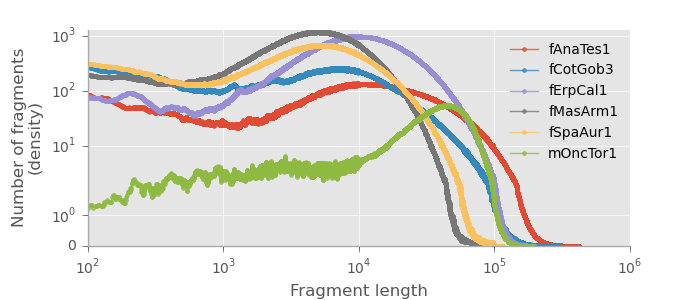
\includegraphics[width=0.9\linewidth]{images/fragmentLength.png}
\captionof{figure}{Density of fragments at longest fragment length (molecule length).}
\end{center}

\begin{center}
\captionsetup{type=figure}
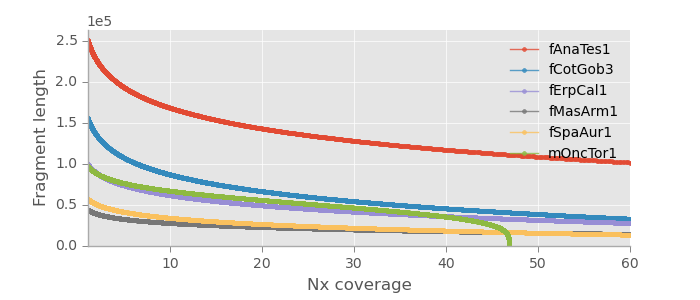
\includegraphics[width=0.9\linewidth]{images/NxCoverage.png}
\captionof{figure}{Longest fragment at Nx coverage.}
\end{center}

{\center\begin{tcolorbox}[boxsep=25pt,width=0.6\linewidth,colback=sangerlightblue3,arc=20pt]
\large\center{
\color{sangertext}
\textbf{www.github.com/pd3/bxcheck}}
\end{tcolorbox}}

\vfill
\columnbreak

%-------------------------------------------------------------------------------
%	3.4.2q40 assembly standard
%-------------------------------------------------------------------------------

\section*{3.4.2q40 assembly standard}

\noindent For the VGP ordinal project and other ``reference quality'' assemblies, we are aiming for a \textbf{3.4.2q40} standard consisting of:

\vspace{0.5cm}

\begin{center}
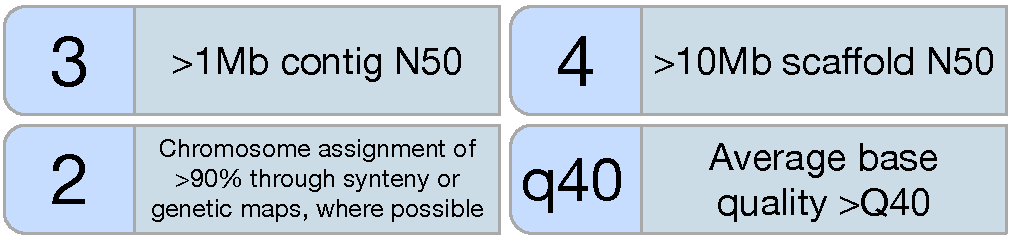
\includegraphics[width=0.6\linewidth]{images/score.pdf}
\end{center}

%-------------------------------------------------------------------------------
%	Assembly progress
%-------------------------------------------------------------------------------

\section*{Assembly progress}

\noindent We have reached our contiguity, scaffolding and base quality goals for 3 of our species so far using just \textbf{PacBio} and \textbf{10X} data. Other species will benefit from additional orthogonal data from \textbf{BioNano Saphyr} and HiC.

\begin{center}
\captionsetup{type=table}
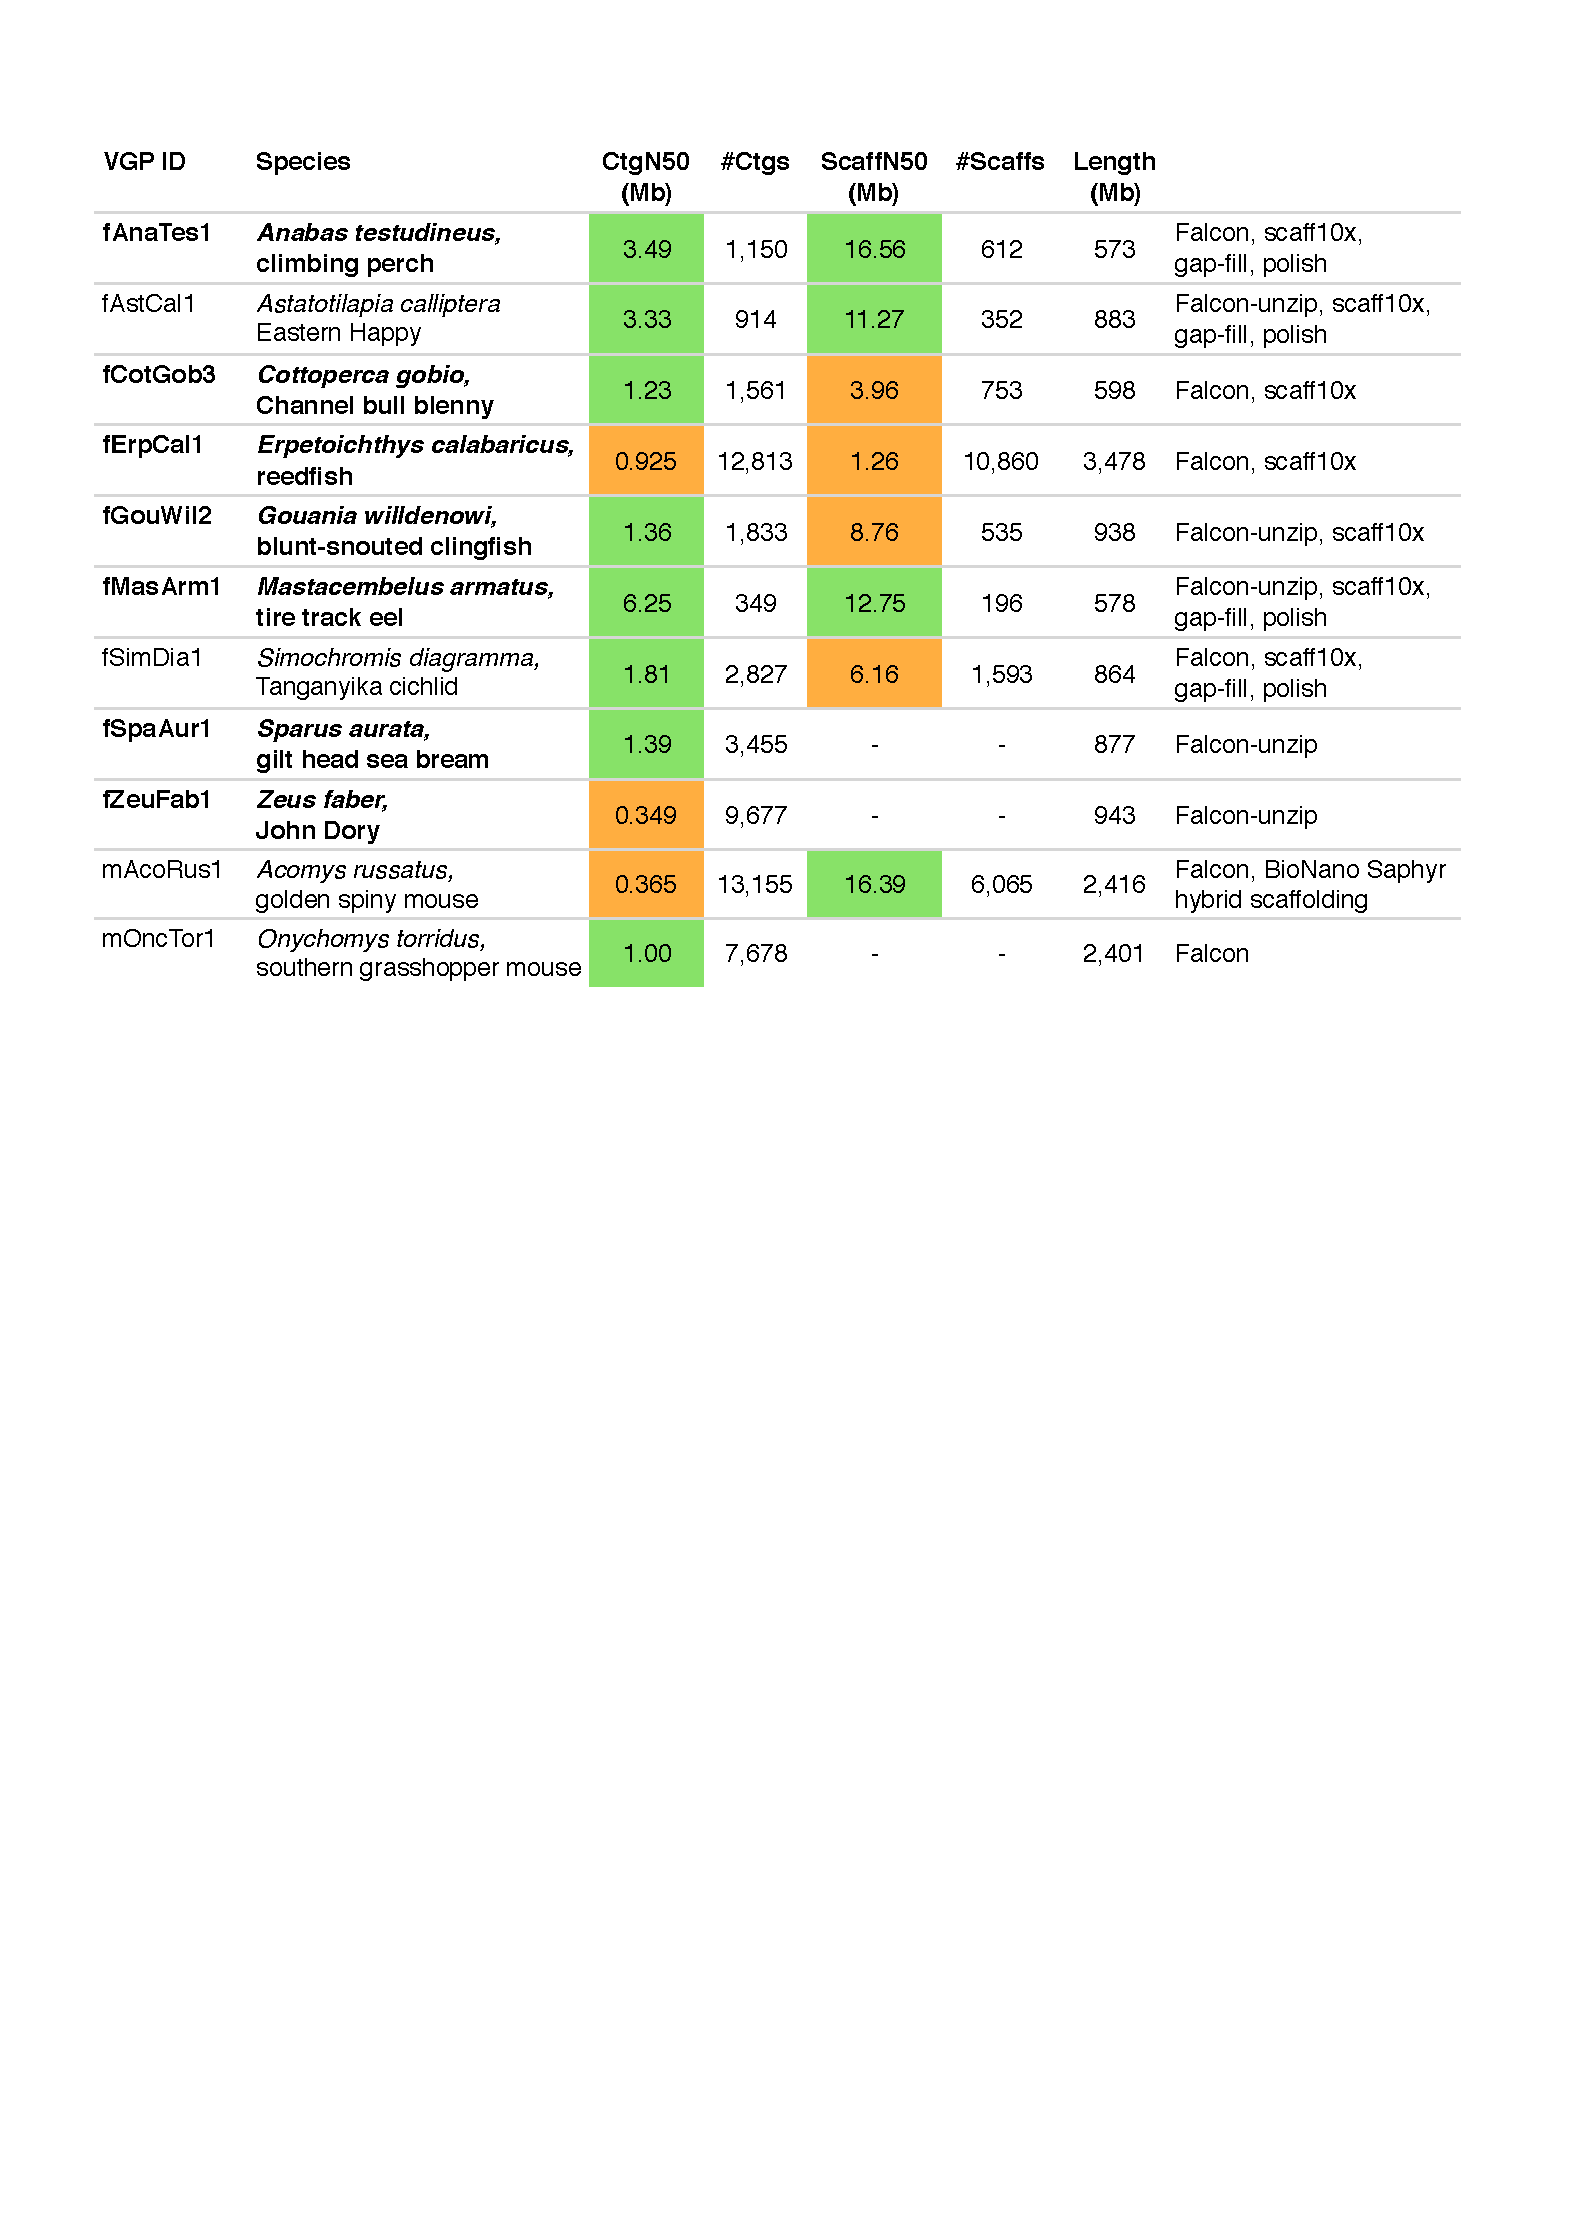
\includegraphics[width=1.0\linewidth]{images/table.pdf}
\captionof{table}{Current status of various PacBio assemblies, showing contig N50, number of contigs, scaffold N50, number of scaffolds and assembly size. Species in bold are those being sequenced as part of the VGP ordinal level project.}
\end{center}

\hfill

\noindent{\textbf{\textcolor{sangertext}{Acknowledgements:}}} {} \small{Byrappa Venkatesh, Maximilian Wagner \textbf{Caecilians}: Mark Wilkinson; \textbf{Cichlids}: George Turner, Martin Genner, Axel Meyer, Walter Salzburger, Milan Malinsky, Alexandra Tyers, Antonia Ford, Craig Albertson; \textbf{Cyprinids}: Lukas Ruber, Ralf Britz, Braedan McCluskey, Andrew Whiteley, Bill Trevarrow, Uwe Irion, Elisabeth Busch-Nentwich, Christiane Nuesslein Vollhard; \textbf{Notothenioids}: Melody Clark, Christina Cheng, Bill Detrich, John Postlethwait, Thomas Desvignes; \textbf{Rodents}: David Thybert, Thomas Keane.}


\end{multicols}

\begin{center}\noindent\rule{1.0\linewidth}{0.05pt}\end{center}

\vfill

\noindent
\begin{minipage}[][][b]{0.75\textwidth}
\begin{tcolorbox}[boxsep=25pt,width=1.0\linewidth,colback=sangerlightblue3,arc=20pt]
\large{
\color{sangertext}
\textbf{www.sanger.ac.uk/science/data/vertebrate-genomes-project
\hfill
sm15@sanger.ac.uk
\hfill
@mcshane
}}
\end{tcolorbox}
\end{minipage}%
\hfill%
\begin{minipage}[][][b]{0.25\textwidth}
    \centering
    
\includegraphics[height=3.75cm]{images/wtsi}
\end{minipage}%

\end{document}